\begingroup
\raggedbottom
\section{更多例子}\label{src:4.9}
\begin{epigraph}
极端的可能情形最能启发人.
\epigraphauthor{David Mumford}
\end{epigraph}
本节给出代数空间 (\S\bookref{4.9.1-subsection}), Deligne--Mumford 叠 (\S\bookref{4.9.2-subsection}) 与代数叠 (\S\bookref{4.9.3-subsection}) 的例子, 以及一些极端不分离的例子 (\S\bookref{4.9.4-subsection}).

\subsection{代数空间的例子}\label{src:4.9.1-subsection}
\begin{example}\label{src:4.9.1}
如例~\bookref{1.5.8} 中所述, 存在一个光滑固有的复三维簇 $U$, 带有 $\mathbb Z/2=\{\pm1\}$ 的自由作用, 且有一个轨道 $\{u,-1\cdot u\}$ 不包含在任何仿射开子概形中. 商层 $X=U/(\mathbb Z/2)$ 是代数空间 (推论~\bookref{4.1.14}), 但不是概形. 若 $X$ 是概形, 则 $u$ 的像具有一个仿射开邻域, 而该开集在有限态射 $U\to X$ 下的原像就是包含该轨道的仿射开集.
\end{example}
\begin{example}[虫眼覆盖]\label{src:4.9.2}
考虑例~\bookref{4.4.4} 中定义的平展等价关系 $(p_2,\sigma):R=(\mathbb Z/2\times\mathbb A^1)\setminus\{(-1,0)\}\rightrightarrows\mathbb A^1$, 它由限制 $\mathbb A^1$ 上的 $\mathbb Z/2$-作用 $(-1)\cdot x=-x$ 得到. 设 $X=\mathbb A^1/R$ 是代数空间商.
\begin{figure}[H]
\centering\begin{tikzcd}[column sep=1.5em,row sep=1.4em]
\mathbb A^1\arrow[d]\arrow[dd,bend right=55,"{x\mapsto x^2}"']&
{\begin{tikzpicture}[baseline=0,x=1cm,y=1cm,font=\small]
\draw (-1.8,.4)..controls (-.3,.3) and (.3,-.3)..(1.8,-.4);
\draw (-1.8,-.4)..controls (-.3,-.3) and (.3,.3)..(1.8,.4);
\fill[red] (1.4,.34) circle (1.6pt);\node[red,above] at (1.4,.34) {$x$};
\fill[red] (1.4,-.34) circle (1.6pt);\node[red,below] at (1.4,-.34) {$-x$};
\node[red,above] (noid) at (-.2,.7) {此处不等同};\draw[red,->] (noid.south)--(0,.04);
\node[red,right] at (1.8,0) {等同};
\end{tikzpicture}}\arrow[d]\\
X\arrow[d]&
{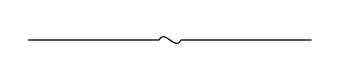
\begin{tikzpicture}[baseline=0,x=1cm,y=1cm]
\draw (-1.8,0)--(-.14,0)..controls (-.07,.15) and (.07,-.15)..(.14,0)--(1.8,0);
\end{tikzpicture}}\arrow[d]\\
\mathbb A^1&
{\begin{tikzpicture}[baseline=0,x=1cm,y=1cm]\draw (-1.8,0)--(1.8,0);\end{tikzpicture}}
\end{tikzcd}

\caption{$X\to\mathbb A^1$ 是虫眼覆盖.}\label{src:4.9.3}
\end{figure}
我们断言代数空间商 $X=\mathbb A^1/R$ 不是概形. 为此, 我们将证明对角线 $X\to X\times X$ 不是局部闭浸入. 这由下列 Cartesian 图得到:
\[
\begin{tikzcd}[column sep=2em]
(\mathbb A^1\setminus0)\amalg\{0\}\arrow[r]\arrow[d]&R\arrow[r]\arrow[d,"{(p_2,\sigma)}"]&X\arrow[d,"\Delta"]\\
\mathbb A^1\arrow[r,"{t\mapsto(t,-t)}"']\arrow[ur,phantom,"\square" description]&\mathbb A^1\times\mathbb A^1\arrow[r]\arrow[ur,phantom,"\square" description]&X\times X,
\end{tikzcd}
\]
因为最左侧的竖直箭头显然不是局部闭浸入.

代数空间 $X$ 光滑且一维, 与仿射直线惊人地相似. 此例最早出现于 \cite[第 $311$ 页]{Art74a}. \newterm{虫眼覆盖}{bug-eyed cover} 这一术语由 \cite[\S$4.2.2$]{Kol92} 提出, 其中考虑了更一般的覆盖: 若 $Y\to Z$ 是概形之间的一般平展态射, 平展轨迹为 $Y^{\text{ét}}$, 则 $Z^{\mathrm{bug}}=Y/R\to Z$ 是虫眼覆盖, 其中
\[
R=Y\amalg\bigl(Y^{\text{ét}}\times_Z Y^{\text{ét}}\setminus\Delta^{\text{ét}}\bigr),
\]
而 $\Delta^{\text{ét}}$ 是 $Y^{\text{ét}}\to Z$ 的对角线.
\end{example}
\begin{exercise}[虫眼覆盖的其他描述]\label{src:4.9.4}
设 $X$ 是上例中的虫眼覆盖.
\begin{enumerate}[(a)]
\item 证明 $X$ 同构于商 $U/(\mathbb Z/2)$, 其中 $U=\mathbb A^1\cup_{\mathbb A^1\setminus0}\mathbb A^1$ 是 $k$ 上的不分离仿射直线, $\mathbb Z/2$ 的自由作用交换两个原点, 且对 $x\ne0$ 作用为 $(-1)\cdot x=-x$.
\item 证明存在万有同胚 $X\to\mathbb A^1$, 它在原点之外为同构, 但在原点上分歧.
\item 证明每个到概形的映射 $X\to Z$ 都经过 $X\to\mathbb A^1$ 分解. (换言之, $\mathbb A^1$ 是概形范畴中 $U$ 对 $\mathbb Z/2$ 的范畴商, 但不是代数空间范畴中的范畴商.)
\item (困难) 考虑 $\operatorname{SL}_2$ 在 $V_d=\operatorname{Sym}^d k^2$ 上的作用, 其中 $V_d$ 是 $x,y$ 的 $d$ 次齐次多项式空间. 设 $W\subseteq V_1\times V_4$ 是由满足 $L\ne0$ 且 $F$ 为判别式等于 $1$ 的齐次二次型的平方的二元组 $(L,F)$ 所定义的约化局部闭子概形. 证明诱导的 $\operatorname{SL}_2$-作用在 $W$ 上自由, 且 $X\cong W/\operatorname{SL}_2$.

虽然把 $X$ 描述为 $\mathbb A^1/R$ 与 $U/(\mathbb Z/2)$ 看起来有些病态, 但此习题说明 $X$ 也可以由拟仿射簇对 $\operatorname{SL}_2$ 取商得到. 另见 \cite[例 $0.4$]{GIT} 和 \cite[例 $2.18$]{Kol97}.
\item (困难) 设 $\pi:Y\to\mathbb A^1$ 是曲面的固有平坦族, 在 $\mathbb A^1\setminus0$ 上光滑. 再假设中心纤维 $Y_0$ 在点 $p$ 处有孤立结点奇点, 局部由 $z^2+xy=t$ 给出, 其中 $t$ 是 $\mathbb A^1$ 的局部坐标. 证明函子
\[
\begin{aligned}
F:(\Sch/\mathbb A^1)&\longrightarrow\mathsf{Sets},\\
(T\to\mathbb A^1)&\longmapsto
\{\text{同时解消 }\widetilde Y\to Y\times_{\mathbb A^1}T\}
\end{aligned}
\]
可由虫眼覆盖 $X$ 表出, 其中\newterm{同时解消}{simultaneous resolution} 是在每个几何纤维上均为极小解消的固有态射. 另见 \cite[第 $331$ 页]{Art74a}.
\end{enumerate}
\end{exercise}
\begin{exercise}\label{src:4.9.5}
设 $V=\Spec k[x,y]/(xy)$, $U=V\cup_{V\setminus0}V$ 是不分离的并. 令 $\mathbb Z/2$ 作用于 $U$, 交换分支并交换两个原点, 设 $X=U/(\mathbb Z/2)$ 为商代数空间.
\begin{figure}[H]
\centering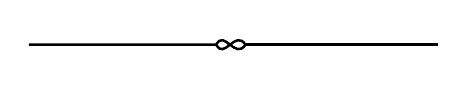
\begin{tikzpicture}[x=1cm,y=1cm]
\draw[line width=.9pt] (-2.6,0)--(-.22,0)
..controls (-.12,.2) and (.02,-.2)..(.15,0)
..controls (.02,.2) and (-.12,-.2)..(-.22,0);
\draw[line width=.9pt] (.15,0)--(2.6,0);
\end{tikzpicture}

\caption{在原点处具有结点奇点的仿射直线.}\label{src:4.9.6}
\end{figure}
\begin{enumerate}[(a)]
\item 证明 $X$ 的对角线不是局部闭浸入, 并由此推出 $X$ 不是概形.
\item 证明 $X$ 一维且在原点处有奇点, 并且存在万有同胚 $X\to\mathbb A^1$, 它在原点之外为同构.
\item 推广此例, 构造一个看起来像在原点处具有 $A_k$ 奇点 (即 $y^2=x^k+1$) 的仿射直线的代数空间.
\item 构造在原点处具有 (非局部完全交) 奇点 $k[[x,y,z]]/(xy,yz,xz)$ (即 $\mathbb A^3$ 中的三条坐标轴) 的仿射直线.
\end{enumerate}
\end{exercise}
\begin{exercise}\label{src:4.9.7}
令 $\mathbb Z/2=\{\pm1\}$ 在 $\Spec\mathbb R$ 上通过共轭作用于 $\mathbb A^1_{\mathbb C}$. 设 $R=(\mathbb Z/2\times\mathbb A^1_{\mathbb C})\setminus\{(-1,0)\}\rightrightarrows U$ 是诱导的平展等价关系. 证明代数空间 $X=\mathbb A^1_{\mathbb C}/R$ 不是概形. 再注意, 与虫眼覆盖和上例不同, $X$ 的对角线是局部闭浸入. (对角线为局部闭浸入的条件有时称为\newterm{局部分离}{locally separated}, 它与 Zariski 局部分离是不同的概念.)

\textit{提示:} 将 $X$ 等同于不分离仿射直线 $U=\mathbb A^1_{\mathbb C}\cup_{\mathbb A^1_{\mathbb C}\setminus0}\mathbb A^1_{\mathbb C}$ 对 $\mathbb Z/2$-作用的商 $U/(\mathbb Z/2)$, 该作用通过共轭作用并交换两个原点. 若原点有一个仿射邻域, 证明其原像将是包含这两个邻域的仿射邻域.
\begin{figure}[H]
\centering\begin{tikzpicture}[x=1cm,y=1cm,font=\small]
\draw[line width=.8pt] (-2.5,0)--(2.5,0);
\shade[ball color=gray] (0,0) circle (2.4pt);
\node[red,below] at (0,-.08) {$\mathbb C$};
\node[red,below] (others) at (1.8,-.55) {其余点的剩余域均为 $\mathbb R$};
\draw[red,->] (others.north)--(1.1,-.03);
\end{tikzpicture}

\caption{商 $X=\mathbb A^1/R$ 看起来像 $\mathbb A^1_{\mathbb R}$, 但原点的剩余域为 $\mathbb C$.}\label{src:4.9.8}
\end{figure}
\end{exercise}
\begin{remark}\label{src:4.9.9}
代数几何中的典型构造往往只在代数空间范畴中存在. 若有限群在概形上的自由作用的每个轨道都包含在一个仿射开集中, 则商作为概形存在 (习题~\bookref{5.2.14}), 但一般情形下并不成立 (例~\bookref{4.9.1}). 类似地, 闭浸入 $X_0\hookrightarrow X$ 与有限 (甚至仿射) 态射 $X_0\to Y_0$ 的推出 $X\amalg_{X_0}Y_0$ 总作为代数空间存在 \cite[定理 $6.1$]{Art70}, 但未必是概形; 例如若 $Y_0$ 中每个点在 $X_0$ 中的原像都包含在一个仿射开集中, 则它是概形 (定理~\bookref{B.4.1}).

Castelnuovo 证明了光滑曲面中自交数为负的曲线可以收缩 (定理~\bookref{B.2.6}), 但高维情形的收缩未必作为概形存在. Artin \cite[定理 $3.1$]{Art70} (另见 \cite{Maz75}) 给出了它们作为代数空间存在的条件. 同样, 曲面族的奇点的同时解消 (如习题~\bookref{4.9.4}(e)) 未必作为概形存在, 但作为代数空间存在 \cite[定理 $1$]{Art74a}.
\end{remark}

\subsection{Deligne--Mumford 叠的例子}\label{src:4.9.2-subsection}
\begin{example}[分类叠]\label{src:4.9.10}
若 $G$ 是域 $k$ 上的有限抽象群概形, 则 $G$ 的分类叠 $BG$ 是以二元组 $(T,P)$ 为对象的叠, 其中 $T$ 是概形, $P\to T$ 是 $G$-torsor (定义~\bookref{3.4.15}). 分类叠 $BG$ 是 $k$ 上光滑固有的零维 Deligne--Mumford 叠.
\end{example}
\begin{example}[简单的例子]\label{src:4.9.11}
假设 $\operatorname{char}(k)\ne2$.
\begin{enumerate}[(a)]
\item 作用 $-1\cdot x=-x$ 的商叠 $[\mathbb A^1/(\mathbb Z/2)]$ 是 $k$ 上光滑的一维 Deligne--Mumford 叠, 它看起来像仿射直线, 但在原点处具有 $\mathbb Z/2$-稳定子. 复合 $\mathbb A^1\to[\mathbb A^1/(\mathbb Z/2)]\to\mathbb A^1$ 是由 $x\mapsto x^2$ 给出的二重覆盖. 后一个映射
\[
[\mathbb A^1/(\mathbb Z/2)]\longrightarrow
\Spec\Gamma(\mathbb A^1,\mathcal O_{\mathbb A^1})^{\mathbb Z/2}
=\Spec k[x^2]=\mathbb A^1
\]
是固有双射, 在原点之外为同构, 并且是粗模空间的一个例子 (见定理~\bookref{5.2.3}).
\item 作用 $(-1)\cdot(x,y)=(y,x)$ 的商叠 $[\Spec(k[x,y]/(xy))/(\mathbb Z/2)]$ 是一维 Deligne--Mumford 叠, 在原点处具有奇点. 然而, 粗模空间
\[
[\Spec(k[x,y]/(xy))/(\mathbb Z/2)]\longrightarrow
\Spec(k[x,y]/(xy))^{\mathbb Z/2}=\Spec k[x+y]=\mathbb A^1
\]
光滑.
\item 作用 $-1\cdot(x,y)=(-x,-y)$ 的商 $[\mathbb A^2/(\mathbb Z/2)]$ 是域 $k$ 上的光滑 Deligne--Mumford 叠. 粗模空间
\[
\begin{aligned}
[\mathbb A^2/(\mathbb Z/2)]&\longrightarrow\Spec k[x,y]^{\mathbb Z/2}\\
&=\Spec k[x^2,xy,y^2]=\Spec k[A,B,C]/(B^2-AC)
\end{aligned}
\]
是奇异锥面.
\end{enumerate}
\end{example}
\begin{example}[拟有限但不有限的惯性]\label{src:4.9.12}
设 $G=\mathbb A^1\amalg(\mathbb A^1\setminus0)\to\mathbb A^1$ 是除原点上的纤维平凡之外每个纤维均为 $\mathbb Z/2$ 的群概形. 则 $BG\to\mathbb A^1$ 是对角线拟有限但不有限的 Deligne--Mumford 叠, 因而不分离. 类似地, $\mathbb P^1$ 中四个无序点的模叠 $[\operatorname{Sym}^4\mathbb P^1/\operatorname{PGL}_2]$ 的 Deligne--Mumford 轨迹不分离 (见例~\bookref{5.4.17}).
\begin{figure}[H]
\centering\begin{tikzpicture}[x=1cm,y=1cm,font=\small]
\draw[gray,line width=4pt,opacity=.3] (-2.5,0)--(2.5,0);
\draw[line width=.6pt] (-2.5,0)--(2.5,0);
\fill[white] (0,0) circle (2pt);
\node[red,below] (nonzero) at (-1.5,-.45) {$\mathbb Z/2$};
\draw[red,->] (nonzero.north)--(-1.8,-.03);
\node[red,below] (zero) at (.7,-.45) {平凡};
\draw[red,->] (zero.north)--(0,-.03);
\end{tikzpicture}

\caption{稳定子群在原点上向下跳跃.}\label{src:4.9.13}
\end{figure}
\end{example}
\begin{example}[加权射影叠]\label{src:4.9.14}
对于正整数元组 $(d_0,\ldots,d_n)$, 令 $\mathbb G_m$ 作用于 $\mathbb A^{n+1}$, 作用为 $t\cdot(x_0,\ldots,x_n)=(t^{d_0}x_0,\ldots,t^{d_n}x_n)$. 定义\newterm{加权射影叠}{weighted projective stack} 为
\[
\mathcal P(d_0,\ldots,d_n)=[(\mathbb A^{n+1}\setminus0)/\mathbb G_m].
\]
若所有 $d_i$ 均为 $1$, 则得到射影空间 $\mathbb P^n$; 否则, $\mathcal P(d_0,\ldots,d_n)$ 不是代数空间. 例如, 在 $\mathbb Z[1/6]$ 上, 稳定椭圆曲线叠 $\overline{\mathcal M}_{1,1}$ 同构于 $\mathcal P(4,6)$, 见习题~\bookref{4.1.21}(b).

更一般地, 若 $R$ 是有限生成的正分次 $k$-代数, 则可以定义\newterm{叠式 Proj}{stacky proj} 为 $\mathcal{P}roj\,R=[(\Spec(R)\setminus0)/\mathbb G_m]$, 其中 $\mathbb G_m$ 的作用使 $x_i$ 的权与其次数相同.
\end{example}
\begin{exercise}\label{src:4.9.15}
\begin{enumerate}[(a)]
\item 若 $k$ 是特征为 $p$ 的域, 证明 $\mathcal P(d_0,\ldots,d_n)$ (更准确地说, $\mathcal P(d_0,\ldots,d_n)\times_{\mathbb Z}k$) 是 $k$ 上的 Deligne--Mumford 叠当且仅当 $p$ 不整除每个 $d_i$.
\item 分类 $\mathcal P(3,3,4,6)$ 中具有非平凡稳定子的所有点.
\item 若存在稠密开子叠 $\mathcal U\subset\mathcal X$ 为代数空间, 则称代数叠 $\mathcal X$ 的\newterm{一般稳定子平凡}{generically trivial stabilizer}. 给出 $\mathcal P(d_0,\ldots,d_n)$ 的一般稳定子平凡的条件.
\item 证明存在从 $\mathcal P(d_0,\ldots,d_n)$ 到加权射影空间 $\operatorname{Proj}k[x_0,\ldots,x_n]$ 的双射态射, 其中 $x_i$ 的次数为 $d_i$. (这是粗模空间的一个例子.)
\end{enumerate}
\end{exercise}
\begin{example}[叠曲线]\label{src:4.9.16}
\newterm{叠曲线}{stacky curve} 是域 $k$ 上有限型的一维 Deligne--Mumford 叠. 对于正整数 $m,n$, 只要特征与 $m,n$ 均互素, 加权射影叠 $\mathcal P(m,n)$ 就是光滑固有叠曲线的一个例子.
\end{example}
\begin{exercise}\label{src:4.9.17}
\begin{enumerate}[(a)]
\item 证明光滑叠曲线的稳定子是 Abel 群.
\item 将此推广到结点叠曲线.
\end{enumerate}
\end{exercise}
\begin{example}[足球曲线]\label{src:4.9.18}
对于整数 $m,n$, \newterm{足球曲线}{football curve} $\mathcal F(m,n)$ 是将 $[\mathbb A^1/\mu_m]$ 与 $[\mathbb A^1/\mu_n]$ 沿
\[
[(\mathbb A^1\setminus0)/\mu_m]\cong\mathbb A^1\setminus0
\cong[(\mathbb A^1\setminus0)/\mu_n]
\]
粘合得到的固有叠曲线. 拓扑空间 $|\mathcal F(m,n)|$ 与 $|\mathbb P^1|$ 等同, 而 $\mathcal F(m,n)\to\mathbb P^1$ 是粗模空间的一个例子.
\end{example}
\begin{exercise}\label{src:4.9.19}
证明 $\mathcal F(m,n)\cong\mathcal P(m,n)$ 当且仅当 $m,n$ 互素.
\end{exercise}
\begin{remark}[叠曲线的单值化]\label{src:4.9.20}
\cite{BN06} 证明了 $\mathbb C$ 上的每条光滑分离叠曲线都有万有覆盖, 该覆盖是一般稳定子平凡的单连通光滑分离叠曲线, 且同构于 $\mathbb H$, $\mathbb C$, 或满足 $\gcd(m,n)=1$ 的 $\mathcal P(m,n)$.
\end{remark}
根 gerbe 与根叠是 Deligne--Mumford 叠的重要例子. 它们最初由 \cite[\S$2$]{Cad07} 引入, 并且可以方便地用非 Deligne--Mumford 叠 $B\mathbb G_m$ 与 $[\mathbb A^1/\mathbb G_m]$ 定义 (见例~\bookref{4.9.24} 与~\bookref{4.9.25}).
\begin{example}[根 gerbe]\label{src:4.9.21}
设 $X$ 是概形, $L$ 是线丛. 这些资料确定态射 $[L]:X\to B\mathbb G_m$. 对正整数 $r$, 设 $r:B\mathbb G_m\to B\mathbb G_m$ 是由 $r$ 次幂映射 $r:\mathbb G_m\to\mathbb G_m$, $t\mapsto t^r$ 诱导的态射; 也可以在线丛对象上通过赋值 $M\mapsto M^{\otimes r}$ 函子性地定义 $r:B\mathbb G_m\to B\mathbb G_m$. 定义 $X$ 与 $L$ 的 \newterm{$r$ 次根 gerbe}{root gerbe} $X(\sqrt[r]{L})$ (有时记为 $\sqrt[r]{L/X}$) 为纤维积
\[
\begin{tikzcd}
X(\sqrt[r]{L})\arrow[r]\arrow[d,"\pi"']&B\mathbb G_m\arrow[d,"r"]\\
X\arrow[r,"{[L]}"']\arrow[ur,phantom,"\square" description]&B\mathbb G_m.
\end{tikzcd}
\]
gerbe 将在 \S\bookref{7.4.3-subsection} 中讨论. 映射 $X(\sqrt[r]{L})\to X$ 是带系 $\mu_r$-gerbe 的一个例子 (习题~\bookref{7.4.26}), 特别地, 它是粗模空间.
\end{example}
\newpage
\begin{example}[根叠]\label{src:4.9.22}
设 $X$ 是概形, $L$ 是线丛, $s\in\Gamma(X,L)$ 是截面. 这些资料确定态射 $[L,s]:X\to[\mathbb A^1/\mathbb G_m]$ (见下面的例~\bookref{4.9.25}). 设 $r:[\mathbb A^1/\mathbb G_m]\to[\mathbb A^1/\mathbb G_m]$ 是由 $r$ 次幂映射 $r:\mathbb A^1\to\mathbb A^1$, $x\mapsto x^r$ 诱导的态射, 该映射对于 $r$ 次幂映射 $r:\mathbb G_m\to\mathbb G_m$ 等变; 也可以在线丛及截面上通过 $(M,t)\mapsto(M^{\otimes r},t^{\otimes r})$ 函子性地定义此态射. 对于正整数 $r$, 定义 $X$ 与 $L$ 沿 $s$ 的 \newterm{$r$ 次根叠}{root stack} $X(\sqrt[r]{L},s)$ (有时记为 $\sqrt[r]{(L,s)/X}$) 为纤维积
\[
\begin{tikzcd}
X(\sqrt[r]{L},s)\arrow[r]\arrow[d,"\pi"']&{[\mathbb A^1/\mathbb G_m]}\arrow[d,"r"]\\
X\arrow[r,"{[L,s]}"']\arrow[ur,phantom,"\square" description]&{[\mathbb A^1/\mathbb G_m]}.
\end{tikzcd}
\]
结构映射 $\pi:X(\sqrt[r]{L},s)\to X$ 是粗模空间的一个例子.

\textit{警告:} 若 $s=0$ 是零截面, 则 $X(\sqrt[r]{L},0)$ 不同构于根 gerbe $X(\sqrt[r]{L})$, 尽管它们具有相同的约化结构和相同的粗模空间.
\end{example}
\begin{exercise}\label{src:4.9.23}
设 $S$ 是概形, $r$ 是在 $\Gamma(S,\mathcal O_S)$ 中可逆的整数. (这一假设保证 $\mu_{r,S}\to S$ 是平展群概形; 习题~\bookref{7.4.26} 将去掉此假设.)
\begin{enumerate}[(a)]
\item 证明 $X(\sqrt[r]{L})$ 与 $X(\sqrt[r]{L},s)$ 是 Deligne--Mumford 叠.
\item 证明 $X(\sqrt[r]{L})$ 具有如下等价描述: 对象为元组 $(f:T\to X,M,\alpha)$, 其中 $f:T\to X$ 是从概形出发的态射, $M$ 是 $T$ 上的线丛, $\alpha:M^{\otimes r}\xrightarrow{\sim}f^*L$ 是同构. 特别地, $X(\sqrt[r]{L})$ 上有线丛 $L^{1/r}$ 及同构 $(L^{1/r})^{\otimes r}\xrightarrow{\sim}\pi^*L$.
\item 证明 $X(\sqrt[r]{L},s)$ 具有如下等价描述: 对象为三元组 $(T\xrightarrow{f}X,M,\alpha,t)$, 其中 $f:T\to X$ 是从概形出发的态射, $M$ 是 $T$ 上的线丛, $\alpha:M^{\otimes r}\to f^*L$ 是同构, $t\in\Gamma(T,M)$ 是满足 $\alpha(t^{\otimes r})=f^*s$ 的截面. 特别地, $X(\sqrt[r]{L},s)$ 上有带截面 $s^{1/r}$ 的线丛 $L^{1/r}$, 以及将 $(s^{1/r})^{\otimes r}$ 与 $\pi^*s$ 等同的同构 $(L^{1/r})^{\otimes r}\xrightarrow{\sim}\pi^*L$.
\item 若 $X=\Spec A$ 是 $S$ 上的仿射概形, 且 $L=\mathcal O_X$ 平凡, 证明
\[
X(\sqrt[r]{L})\cong[X/\mu_r],\qquad
X(\sqrt[r]{L},s)\cong[\Spec(A[x]/(x^r-s))/\mu_r],
\]
其中 $\mu_r$ 在 $X$ 上平凡作用, 并通过 $t\cdot x=tx$ 作用于 $\Spec(A[x]/(x^r-s))$.
\item 证明 $X(\sqrt[r]{L})\to X$ 在点 $x\in X$ 上的纤维同构于 $B\mu_{r,\kappa(x)}$.
\item 证明 $X(\sqrt[r]{L},s)\to X$ 在 $X_s=\{s\ne0\}$ 上为同构, 而在 $V(s)$ 上限制为根 gerbe $V(s)(\sqrt[r]{L|_{V(s)}})$ 的无穷小扩张.
\end{enumerate}
\end{exercise}

\subsection{代数叠的例子}\label{src:4.9.3-subsection}
\begin{example}\label{src:4.9.24}
$\Spec\mathbb Z$ 上的分类叠 $B\operatorname{GL}_n$ 分类秩为 $n$ 的向量丛. 当 $n=1$ 时, $B\mathbb G_m=B\operatorname{GL}_1$ 分类线丛. 叠 $B\operatorname{GL}_n$ 是 $\Spec\mathbb Z$ 上普遍闭且光滑的代数叠, 相对维数为 $-n^2$, 并具有仿射对角线. 然而, $B\operatorname{GL}_n$ 既不分离, 也不是 Deligne--Mumford 叠. 结构态射 $B\operatorname{GL}_n\to\Spec\mathbb Z$ 是粗模空间与平凡带系 $\operatorname{GL}_n$-gerbe 的一个例子.
\end{example}
\begin{samepage}
\begin{example}\label{src:4.9.25}
若 $\mathbb G_m$ 在 $\Spec\mathbb Z$ 上通过伸缩作用于 $\mathbb A^1$, 则商叠 $[\mathbb A^1/\mathbb G_m]$ 在概形 $T$ 上的对象为二元组 $(L,s)$, 其中 $L$ 是 $T$ 上的线丛, $s\in\Gamma(T,L)$. 叠 $[\mathbb A^1/\mathbb G_m]$ 是 $\Spec\mathbb Z$ 上普遍闭且光滑的代数叠, 相对维数为 $0$, 并具有仿射对角线. 然而, 它既不分离, 也不是 Deligne--Mumford 叠. 在域 $k$ 上, $[\mathbb A^1/\mathbb G_m]$ 有两个点, 一个开点和一个闭点, 对应于两个 $\mathbb G_m$-轨道 (见图~\bookref{1.4.7}). 存在开浸入与闭浸入
\[
\begin{tikzcd}
1:\Spec k\arrow[r,hook,"\text{开}"]&{[\mathbb A^1/\mathbb G_m]}&B\mathbb G_m:0\arrow[l,hook',"\text{闭}"'].
\end{tikzcd}
\]
态射 $[\mathbb A^1/\mathbb G_m]\to\Spec k$ 将两个轨道等同, 是良模空间的一个例子.
\end{example}
\end{samepage}
\begin{exercise}\label{src:4.9.26}
证明 $[\mathbb P^1/\mathbb G_m]\cong[(\mathbb A^1\cup_{\mathbb A^1\setminus0}\mathbb A^1)/\mathbb G_m]$.
\end{exercise}
\begin{example}\label{src:4.9.27}
在域 $k$ 上, 作用 $t\cdot[x:y]=[x+ty:y]$ 的商叠 $[\mathbb P^1/\mathbb G_a]$ 有两个点, 一个开点和一个闭点:
\[
\begin{tikzcd}
0:\Spec k\arrow[r,hook,"\text{开}"]&{[\mathbb P^1/\mathbb G_a]}&B\mathbb G_a:\infty\arrow[l,hook',"\text{闭}"'].
\end{tikzcd}
\]
\end{example}
\begin{example}\label{src:4.9.28}
在域 $k$ 上, 令 $\mathbb G_m$ 通过 $t\cdot(x,y)=(tx,t^{-1}y)$ 作用于 $\mathbb A^2$. 商叠 $[\mathbb A^2/\mathbb G_m]$ 是一维光滑代数叠. 它在概形 $T$ 上的对象为三元组 $(L,s,t)$, 其中 $L$ 是 $T$ 上的线丛, $s\in\Gamma(T,L)$, $t\in\Gamma(T,L^{-1})$. 原点的补 $[\mathbb A^2/\mathbb G_m]\setminus0$ 同构于不分离仿射直线. 存在由 $(x,y)\mapsto xy$ 定义的态射 $\pi:[\mathbb A^2/\mathbb G_m]\to\mathbb A^1$, 它在 $\mathbb A^1\setminus0$ 上为同构, 并将 $xy=0$ 定义的三个轨道等同; 这是良模空间的一个例子.
\begin{figure}[H]
\centering\refstepcounter{figure}\label{src:4.9.29}
% Source printed p. 161, 400 DPI. Preserve the original uncaptioned illustration.
\begin{tikzpicture}
\node[anchor=south west,inner sep=0] (art) at (0,0)
{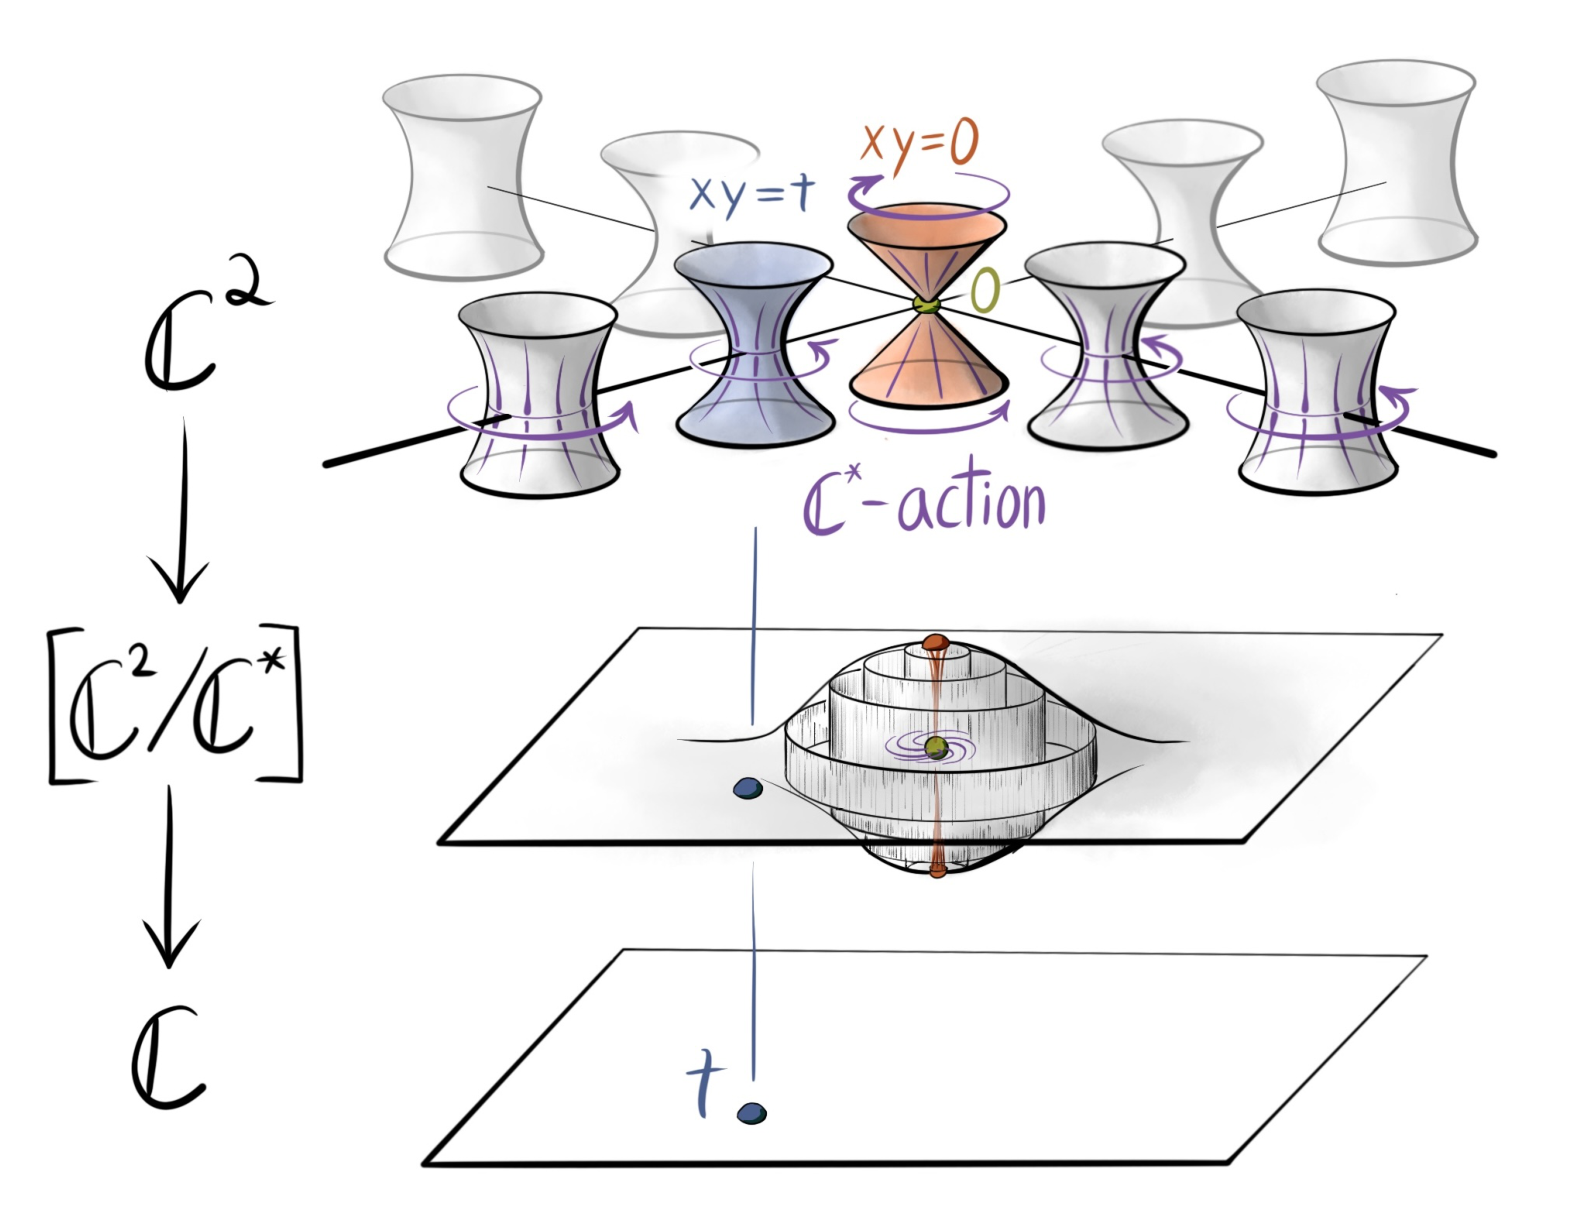
\includegraphics[width=.64\textwidth]{figures/fig-4.9.29.png}};
\begin{scope}[x={(art.south east)},y={(art.north west)}]
\fill[white] (0,0) rectangle (.205,1);
\node at (.105,.44) {\begin{tikzcd}[row sep=4.8em]
\mathbb C^2\arrow[d]\\
{[\mathbb C^2/\mathbb C^*]}\arrow[d]\\
\mathbb C
\end{tikzcd}};
\fill[white] (.50,.557) rectangle (.68,.628);
\node[text=violet,font=\small] at (.59,.593) {$\mathbb C^*$-作用};
\end{scope}
\end{tikzpicture}

\end{figure}
\end{example}
\begin{exercise}[表示叠]\label{src:4.9.30}
设 $G$ 是有限生成群, $n$ 是正整数.
\begin{enumerate}[(a)]
\item 定义 $\Gamma$ 的 $n$ 维表示叠 $\operatorname{Rep}_{\Gamma,n}$, 并证明它是代数叠.
\item 若 $\Gamma$ 是有 $\gamma$ 个生成元的自由群, 证明 $\operatorname{Rep}_{\Gamma,n}\cong[\operatorname{GL}_n^\gamma/\operatorname{GL}_n]$, 其中 $\operatorname{GL}_n$ 通过同时共轭作用.
\item 若 $\Gamma=\pi_1(\Sigma)$, 其中 $\Sigma$ 是亏格为 $g$ 的紧 Riemann 曲面, 证明
\[
\operatorname{Rep}_{\Gamma,n}\cong
\left[\left\{(\alpha_i,\beta_i)\in(\operatorname{GL}_n^2)^g\ \middle|\
\prod_{i=1}^g[\alpha_i,\beta_i]=1\right\}/\operatorname{GL}_n\right].
\]
\end{enumerate}
\end{exercise}
\begin{example}[环面叠]\label{src:4.9.31}
格 $L=\mathbb Z^n$ 上的扇 $\Sigma$ 定义环面簇 $X(\Sigma)$, 即带有 $\mathbb G_m^n$-作用且存在稳定子平凡的稠密轨道的正规分离簇; 见 \cite{Ful93}. 另一方面, \newterm{叠式扇}{stacky fan} 是二元组 $(\Sigma,\beta)$, 其中 $\Sigma$ 是格 $L$ 上的扇, $\beta:L\to N$ 是格之间的同态. 由于 $L,N$ 是格 (即有限生成自由 Abel 群), 它们的 $\mathbb Z$-线性对偶定义环面 $T_L:=D(L^\vee)$ 与 $T_N:=D(N^\vee)$ (例~\bookref{B.1.7}), 其中 $T_L$ 是环面簇 $X(\Sigma)$ 的环面. 映射 $\beta$ 诱导同态 $T_\beta:T_L\to T_N$, 自然地将 $\beta$ 与单参数子群格上的诱导映射等同. 于是可以定义 $G_\beta=\ker(T_\beta)$ 及\newterm{环面叠}{toric stack}
\[
\mathcal X(\Sigma,\beta):=[X(\Sigma)/G_\beta].
\]
与环面簇的作用类似, 环面叠提供了丰富的组合例子, 可以用来检验一般猜想. 见 \cite{FMN10,GS17}.
\end{example}
\begin{example}[Picard 概形与叠]\label{src:4.9.32}
设 $X$ 是代数闭域 $k$ 上的固有整概形. $X$ 的 Picard 函子与 Picard 叠定义为 $\Sch_{\text{ét}}$ 上的层 $\underline{\operatorname{Pic}}(X)$ 与叠 $\mathcal{P}ic(X)$:
\[
\begin{aligned}
\underline{\operatorname{Pic}}(X)&=\text{函子 }T\longmapsto\operatorname{Pic}(X_T)\text{ 的层化},\\
\mathcal{P}ic(X)(T)&=\{X_T\text{ 上的线丛 }L\text{ 组成的群胚}\}.
\end{aligned}
\]
$\mathcal{P}ic(X)$ 中的态射 $(T,L)\to(T',L')$ 由概形态射 $f:T\to T'$ 及同构 $\alpha:L\to f^*L'$ 给出. 层 $\underline{\operatorname{Pic}}(X)$ 可由射影概形表出, 而线丛的张量积赋予它群概形结构, 因而它是 Abel 簇. 此外, $\mathcal{P}ic(X)$ 是 $k$ 上的光滑代数叠. 忘掉自同构群的映射 $\mathcal{P}ic(X)\to\underline{\operatorname{Pic}}(X)$ 是带系 $\mathbb G_m$-gerbe 的一个例子. 见 \S\bookref{7.4.8-subsection}.
\end{example}
\begin{example}[向量丛叠]\label{src:4.9.33}
设 $K^\bullet:K^0\xrightarrow{d}K^1$ 是概形 $X$ 上的两项向量丛复形. \newterm{向量丛叠}{vector bundle stack} $\mathfrak C(K^\bullet)$, 有时称为\newterm{锥叠}{cone stack}, 并记为 $[K^1/K^0]$ 或 $[h^0/h^1]$, 定义为 $(\Sch/X)_{\text{ét}}$ 上的商叠
\[
\mathfrak C(K^\bullet)=[\mathbb A(K^{1,\vee})/\mathbb A(K^{0,\vee})],
\]
其中将 $\mathbb A(K^{0,\vee})$ 视为加法群概形, 作用 $\sigma:\mathbb A(K^{0,\vee})\times\mathbb A(K^{1,\vee})\to\mathbb A(K^{1,\vee})$ 定义为 $\sigma(x_0,x_1)=x_1+d(x_0)$. 当 $X=\Spec k$ 且 $k$ 是域时, $\mathfrak C(K^\bullet)(k)$ 是对象为 $\mathbb A(K^{1,\vee})(k)=K^1$ 的群胚, 态射 $v\to v'$ 是满足 $d(\alpha)=v-v'$ 的元素 $\alpha\in\mathbb A(K^{0,\vee})(k)=K^0$. 此外, $\mathfrak C(K^\bullet)$ 与平凡作用的商 $[\mathbb A(H^1(K^\bullet)^\vee)/\mathbb A(H^0(K^\bullet)^\vee)]$ 等同, 特别地, 群胚 $\mathfrak C(K^\bullet)(k)$ 等价于 $[H^1(K^\bullet)/H^0(K^\bullet)]$.

对一般的 $X$, $\mathfrak C(K^\bullet)\to X$ 在几何点 $\Spec k\to X$ 上的纤维为
\[
\mathfrak C(K^\bullet\otimes_{\mathcal O_X}k)\cong
[\mathbb A(H^1(K^\bullet\otimes_{\mathcal O_X}k)^\vee)/
\mathbb A(H^0(K^\bullet\otimes_{\mathcal O_X}k)^\vee)].
\]
若 $g:T\to X$ 是从仿射概形出发的态射, 则由于 $T$ 上的主 $\mathbb A(K^{0,\vee})$-丛的同构类与 $H^1(T,K^{0,\vee})=0$ 一一对应, 每个主丛均平凡. 因而
\[
\begin{aligned}
\mathfrak C(K^\bullet)(T)
&=[\mathbb A(K^{1,\vee})(T)/\mathbb A(K^{0,\vee})(T)]\\
&\cong[H^0(T,g^*K^1)/H^0(T,g^*K^0)],
\end{aligned}
\]
这里使用了双射
\begin{equation}\label{src:4.9.34}
\begin{aligned}
\mathbb A(K^{i,\vee})(T\xrightarrow{g}S)
&=\operatorname{Mor}_S(T,\mathbb A(K^{i,\vee}))\\
&=\operatorname{Hom}_{\mathcal O_S\text{-}\mathrm{alg}}
(\operatorname{Sym}^*K^{i,\vee},g_*\mathcal O_T)\\
&=\operatorname{Hom}_{\mathcal O_S}(K^{i,\vee},g_*\mathcal O_T)\\
&=H^0(S,K^i\otimes g_*\mathcal O_T)\\
&=H^0(S,g_*g^*K^i)\qquad\text{(投影公式)}\\
&=H^0(T,g^*K^i).
\end{aligned}
\end{equation}
由构造, $\mathfrak C(K^\bullet)\to X$ 是光滑态射, 对任意 $k$-值点 $\Spec k\to X$, 相对维数为 $h^1(K^\bullet\otimes_{\mathcal O_X}k)-h^0(K^\bullet\otimes_{\mathcal O_X}k)$.
\end{example}
\begin{exercise}\label{src:4.9.35}
证明概形 $X$ 上的两项复形之间的拟同构 $K^\bullet\to L^\bullet$ 诱导向量丛叠之间的同构 $\mathfrak C(K^\bullet)\xrightarrow{\sim}\mathfrak C(L^\bullet)$.
\end{exercise}
上面的习题说明, 对振幅在 $[0,1]$ 内的复形 $K^\bullet\in D^b(X)$, 向量丛叠 $\mathfrak C(K^\bullet)$ 是良定义的. 我们将在命题~\bookref{9.2.13} 中用此构造描述 $C\times S$ 上向量丛 $F_1,F_2$ 的扩张叠 $\mathfrak C(Rp_{2,*}\mathcal H om_{\mathcal O_{C\times S}}(F_1,F_2))\to S$, 其中 $C$ 是\mbox{光滑曲线}. 对于 syntomic 态射 $X\to Y$, $L_{X/Y}$ 是振幅在 $[-1,0]$ 内的完美复形, 可以考虑向量丛叠 $\mathfrak C(L_{X/Y}^\vee)$, 它在 \cite{BF97} 中内蕴法锥的定义中起作用.

\subsection{极端不分离的例子}\label{src:4.9.4-subsection}
下面的例子常常提供反例: 某些性质对具有分离且拟紧对角线的代数叠成立, 但在一般情形下失效. 例如, 若 Deligne--Mumford 叠的对角线拟紧且分离, 则它拟仿射 (推论~\bookref{5.5.8}), 特别地可由概形表出; 下面的例子说明拟紧性与分离性两个假设都不可少.
\begin{example}[对角线不拟紧的 Deligne--Mumford 叠]\label{src:4.9.36}
设 $\underline{\mathbb Z}$ 表示 $\Spec\mathbb Z$ 上与抽象离散群 $\mathbb Z$ 对应的常群概形. 分类叠 $B\underline{\mathbb Z}$ 是零维光滑代数叠, 其对角线不拟紧. 特别地, $B\underline{\mathbb Z}$ 不拟分离.

在特征为零的域 $k$ 上, 令 $\mathbb Z$ 作用于 $\mathbb A^1$, 对 $x\in\mathbb A^1$ 与 $n\in\mathbb Z$, 作用为 $n\cdot x=x+n$. 商 $G:=\mathbb A^1/\mathbb Z$ 是拟紧且局部 Noether 的群代数空间, 其对角线不拟紧, 且它不是概形. 域 $k$ 上每个局部有限型的拟分离群代数空间都是概形 (定理~\bookref{5.5.28}), 而此例说明拟分离性假设不可少.

分类叠 $BG$ 是 Deligne--Mumford 叠, 其对角线 $\Delta_{BG}$ 拟紧, 但二重对角线 $\Delta_{\Delta_{BG}}$ 不拟紧; 特别地, $BG$ 不拟分离. 此外, $BG$ 的对角线不可由概形表出.

类似地, 可以考虑代数空间商 $\mathbb A^1_{\mathbb C}/\mathbb Z^2$, 其中 $(a,b)\cdot x=x+a+ib$. 虽然此作用的解析商 $\mathbb C/\mathbb Z^2$ 是 $\mathbb C$ 上的椭圆曲线, 但代数空间商不拟分离, 也不是概形.
\end{example}
\begin{exercise}\label{src:4.9.37}
设 $G=\mathbb A^1/\mathbb Z$.
\begin{enumerate}[(a)]
\item 证明 $G$ 不是概形.
\item 证明一般点 $\Spec k(x)\to\mathbb A^1\to X$ 在 $\mathbb Z$-作用下不变, 且复合 $\Spec k(x)\to G$ 不能经过从某个域 $L$ 出发的单态射 $\Spec L\to G$ 分解, 即 $G$ 的一般点没有剩余域.
\end{enumerate}
\end{exercise}
\begin{example}[对角线不分离的 Deligne--Mumford 叠]\label{src:4.9.38}
不分离仿射直线 $Q:=\mathbb A^1\cup_{\mathbb A^1\setminus0}\mathbb A^1$ 是 $\mathbb A^1$ 上的群概形, 除原点上外每个纤维都平凡. 分类叠 $BQ$ 是对角线不分离的 Deligne--Mumford 叠.

下面给出产生类似例子的构造. 设 $G\to S$ 是有限平展群概形. 若 $H\subseteq G$ 是 $S$ 上的子群概形, 则 $G/H$ 分离当且仅当 $H\subset G$ 闭. 若 $H$ 在 $G$ 中正规, 则 $G/H\to S$ 是群代数空间. 例如, 取 $G=\mathbb Z/2\times\mathbb A^1\to\mathbb A^1$ 及子群 $H=G\setminus\{-1,0\}$, 则商 $Q=G/H$ 是 $\mathbb A^1$ 上的不分离仿射直线.

类似地, 考虑 $\mathbb Q$ 上的 $\mu_{3,\mathbb Q}=\Spec\mathbb Q\amalg G'$, 其中 $G'=\Spec\mathbb Q[x]/(x^2+x+1)$ 是非单位分支, 并令 $G=\mu_{3,\mathbb Q}\times\mathbb A^1_{\mathbb Q}$. 则 $Q=(\mu_{3,\mathbb Q}\times\mathbb A^1_{\mathbb Q})/H$ 是 $\mathbb A^1_{\mathbb Q}$ 上的不分离平展群代数空间, 且不是概形. 它不是概形的原因与习题~\bookref{4.9.7} 类似: $Q\to\mathbb A^1$ 是群概形
\[
\mathbb A^1_{\mathbb Q}\cup_{\mathbb A^1_{\mathbb Q}\setminus0}
\mathbb A^1_{\mathbb Q}\cup_{\mathbb A^1_{\mathbb Q}\setminus0}\mathbb A^1_{\mathbb Q}
\]
的一个形式, 该群概形除原点上的纤维为 $\mathbb Z/2$ 外均平凡. 若 $Q_0$ 中的非单位点包含于一个仿射开集, 则其在 $\mathbb A^1_{\mathbb Q[x]/(x^2+x+1)}\to\mathbb A^1_{\mathbb Q}$ 下的原像是包含其中两个原点的仿射开集, 矛盾.

此时, $BQ$ 是拟紧且拟分离的 Deligne--Mumford 叠 (即 $BG$, 一重对角线 $\Delta_{BG}$ 与二重对角线 $\Delta_{\Delta_{BG}}$ 都拟紧), 但其对角线不分离且不可由概形表出.
\end{example}
虽然模理论中出现的绝大多数代数叠都具有分离对角线, 但也有少数例外, 例如对数结构叠 $\operatorname{Log}_{\mathrm{alg}}$ \cite{Ols03}.
\par\clearpage
\endgroup
